% !TeX encoding = UTF-8
\documentclass{mcmthesis}

\usepackage{ctex}
\usepackage{tabularx}
\usepackage{bigstrut}
\usepackage{makecell}

% 定义图片, 表格, 公式引用命令(也可以直接用\ref, 但不是很好看)
\newcommand*{\figref}[1]{{\bf Figure~\ref{#1}}}
\newcommand*{\tabref}[1]{{\bf Table~\ref{#1}}}
\newcommand*{\equref}[1]{{\bf Equation~\eqref{#1}}}

% 设置一个插图存放目录
\graphicspath{{figures/}}
    
% 模板设置
\mcmsetup{
    tcn = 53889, %队伍控制号码
    problem = C, %选题
    sheet = true, %为真时将输出摘要页
    titleinsheet = true, %为真时将在摘要页输出标题
    keywordsinsheet = false, %为真时将在摘要页输出关键字
    titlepage = true, %为真时将输出标题页
    abstract = false %为真时将在标题页输出摘要和关键词
    }
    
    
\usepackage{mwe}
% 论文标题
%\title{The Template for MCM Version \MCMversion}
% 作者
%\author{names}

\date{\today}


\begin{document}
    % Abstract
    \begin{abstract}
In this article, we adopt an optimal investment strategy which identifies schools, investment amount per school, return on that investment(ROI), and time duration.\par
The first step is to analyze and process the data the problem provides. It appears a number of ''NULL'' results, which is defined as the lack of properties in some schools rather than missing data. We employ Principal Component Analysis (PCA) to reduce dimensions of big data and get some principal components. Then combining with ROI and funds utilization, we formulate an evaluation model based on Analytical Hierarchy Process (AHP) to obtain the primary list of candidate schools.\par
We regard ROI as the degree of graduates’ contributions to society. Combining with the data we capture, we define a formula for ROI. We calculate the ROI of every school and get a list. The Texas A \& M University-College Station is the first.\par
We build an investment portfolio optimization model to determine the investment schools and the investment amount per school with particle swarm algorithm(PSO). In order to analyze the problem explicitly, we build a basic model. We hypothesis that the time duration for investment of all schools is five years. Then we formulate a multi-objective optimization model. Through the method of PSO, we get the strategy for investment and conclude that the number of schools is 227 and Ohio State University-Main Campus gets the most investment that is 1.1 million. \par
We extend our basic model with taking the change of time duration into consideration. We divide the time duration into five parts. The time duration of each school decides on its ROI. The relationship among variables becomes more complicate. So we build a portfolio investment dynamic model. This model takes all the relation into consideration to increase the reliability of our results. From the results, we find time duration of the Texas A \& M University-College Station is five years. You can see the appendix for the information in detail.\par
We conduct a sensitivity analysis for our model finding ROI has a good stability to graduates’ income. Furthermore, the portfolio investment model is largely affected by the increasing investment schools, which needs to be improved.\par
We write a letter to the Chief Financial Officer (CFO) of the Goodgrant Foundation, Mr. Alpha Chiang. It describes our modeling approach and major results.\par


        %\lipsum[1]
        \begin{keywords}
            keyword1; keyword25
        \end{keywords}
    \end{abstract}
%    \maketitle

\newpage
\newpage

% ------------------
% 先把图放在这儿

% ------------------







\section{Introduction}
\subsection{Problem Analysis}
we understand this issue as a problem about investment portfolio according to the majority of topic, not only that ,we need to appropriately provide a definition about return on investment (ROI),which should meet the need of the Goodgrant Foundation. Here, we think that ROI is a reflection of the social value the college graduates produce. At the same time, identifying the schools, the investment amount per school, the return on that investment, and the time duration should be enclosed in an optimal investment strategy we give by taking advantage of the present data. Eventually, we should also write a letter about investment strategy to Mr. Alpha Chiang.\par

In order to give a definition about ROI, we determine the factors affecting ROI by consulting reference materials, then we formulate a synthetic evaluation model based on the standard of return on investment and effectiveness of funds. Subsequently, a short list about investment on schools can be got by ranking. Moreover, we could build a pseudo-portfolio model to distribute funds to the candidate school by employing the return on investment and fund utilization rate.\par

As for the duration time ,we can get the return on investment variation with time using several years of statistical data to determine the duration of the best investments.\par

\subsection{Previous Research}
Endowment income as an important financing channel from sources of education funds has attracted great attention in American high schools. However, it seems especially important in how to allocate finance and identify the school to generate the maximum ROI. How do we measure the return on investment for donations in terms of operators of foundation? It is a very profound knowledge because what the charitable donations refer to is not only direct economic benefits ,but invisible social benefits. Stanley E. Fawcett and Matthew A. Wallers point out that society is looking for a return on its investment—even a reinvention of the university$^{[\ref{1}]}$. Now a revolution has begun, thanks to three forces: rising costs, changing demand and disruptive technology. The result will be the reinvention of the university.$^{[\ref{2}]}$.\par

In our paper, we place emphasis on the definition of RIO and formulate a model to determine an optimal investment strategy that identifies the schools, the investment amount per school, the return on that investment, and the time duration ,solving the problem step by step.\par


\subsection{Outline of Our Model}
To improve the feasibility of the model, the first step is to preprocess the data about information of 2977 schools. It is found that 41 schools are ruled out due to the lack of data, then we screen the indexes of all the schools preliminary and ensure the indexes related to ROI and fund utilization rate. \par

The screened data is used to analyze the correlation in order to reduce dimensions by the PCA, and we combine the advantages of AHP and FSE to build a model for get the evaluation results, a short list of aided schools being out.\par

We will make investments in the schools which are high ROI and fund utilization rate by calculating. Furthermore, funds needs to be properly allocated for schools, so we formulate a pseudo-portfolio model to get the optimal solution with hybrid particle swarm optimization algorithm. Considering the duration, we eventually obtain the ROI of every school in several years using data, and carry out the fitting the ROI with time variation. Hence, we could judge the duration of investment by fitting results representing maximized ROI.\par


%2.假设
\section{Hypothesis}
\begin{itemize}
    \item  Assuming that data collected is accurate and reliable, and can reflect real conditions preferably.
    %假设我们排除的学校不影响最终的排名.经过我们对比题目所给的数据,有41所高校没有任何数据.我们无法对着41所高校做出评价.所以我们舍弃这些学校.
    \item We assume that the schools we rule out do not have an impact on the last ranks considering the 41 schools with the lack of data so that we could not make a comment on these schools. 
    %假设数据筛选后不影响整体的解释性.为了简化问题分析和模型建立,我们从主观判断上删除一些无用的指标.
    \item The filtered data do not have effects on the explanations of the whole and we delete some indexes according to our subjective judgment in order to simplify analysis and model building. 
\end{itemize}\par


%3.数据处理
\section{Data processing}
\subsection{Collecting And Sorting out}
The problem C provides data of 2977 candidate schools. The CollegeScorecardData  has 7804 schools' data. We sort out the data of candidate schools by the ID. We find that there are 41 school don't have data. So we try to get these data from the IPEDS. The IPEDS provides various reports and the statistical data, which include year and statistical variable. Because of the types of the data classified difficultly, we download all the data of the IPEDS. Then we sort them out seriously.\par


\begin{figure}[h]
    \centering
    \includegraphics[width=\linewidth]{figure/number-of-potential-candidate-school}
    \caption{the distribution of potential candidate institution}
    \label{fig:map}
\end{figure}

We get 913 data files from IPEDS eventually. We use ID to matching the 41 schools, which don't have data. From the analysis result we can know that, the data is missing seriously. The analysis result is showed below:

	\begin{table}[h] \renewcommand\arraystretch{1.5}
        \begin{center}
            \begin{footnotesize}
                \begin{tabular}{cccc}
                    \toprule
                    Data Deficiency &Data Error& Data Integrity&Total\\
                    903             &7         &3              &913  \\\bottomrule
                \end{tabular}%
            \end{footnotesize}
            \caption{\footnotesize {Data Integrity report}}
            
        \end{center}
    \end{table}	

There are many "null" and "PrivacySuppressed" among the data the problem provides. We call them "missing data". Through analyzing the data carefully, we know that this situation is result from the different institutions, which have different attributes such as the educational system respectively. We divide the schools into different types according to their attributes. 

	\begin{table}[h] \renewcommand\arraystretch{1.5}
        \centering\
        \begin{footnotesize}
            \newcolumntype{V}{!{\vrule width 1pt}}
            \begin{tabular}{Vc|c|cV}\Xhline{1pt}
                \multirow{2}*{Data For the Ranking}
                &Four-year institutions&1896\\\cline{2-3}
                &Less-than-four-year institutions&1007\\\hline
                \multirow{3}*{Discarded Data}
                &Data Missing&41\\\cline{2-3}
                &No Runing& 8  \\\cline{2-3}
                &Unknown Type&25\\\hline
                \multicolumn{2}{Vc|}{Amout}&2977\\\Xhline{1pt}
                
            \end{tabular}
        \end{footnotesize}
        \caption{\footnotesize {The final Data and Statistics}}
        
    \end{table}
    %加载宏包makecell	

\subsection{Feature Extraction based on PCA(Principal component analysis)}
We extract 28936 data in all about the candidate schools from the CollegeScorecardData. We exclude some schools which are not open according to the variable "CURROPER". Eventually there are 2936 schools ranking. The data in the CollegeScorecardData are not able to be used for calculating. We exclude these indexes which is useless for us. We get 98 variables in the end,
For integrating the data, we use PCA algorithm to process them. The derailed process of PCA are as follows: 
%主成分分析过程
From the results, we can know that we could select 14 principal components, whose contribution rate reach to 99\%.


\section{4.模型建立及求解}
\subsection{4.1 确定候选名单的模型}
%4.1.1层次分析法模型
\subsubsection{Analytic Hierarchy Process Model}
%题目要求通过回报率和资金利用率来确定投资候选名单.而回报率与资金利用率是和更加具体的指标有关系的.所以我们采用了三层结构的层次分析法求解问题.
The problem needs us to determine the candidate school list by return on investments and fund utilization rate, which have something to do with some factors, so we employ AHP with three-level hierarchy structure as the way combining the weighting coefficients of all the factors in the evaluation system to obtain rankings.\par
The specific process of analytic hierarchy process is described in the following procedure.\par
层次分析法具体过程如下:
\begin{itemize}
    % 建立递阶层次结构模型
    \item[Step1]Building hierarchical structural model
    %    通过查阅相关资料、文献,我们建立了层次模型,结果如下图所示:
    We determine the structural model through investigating materials, the result can be seen as followed:
    
    %层次结构图
    
    \begin{figure}[h]
        \centering
        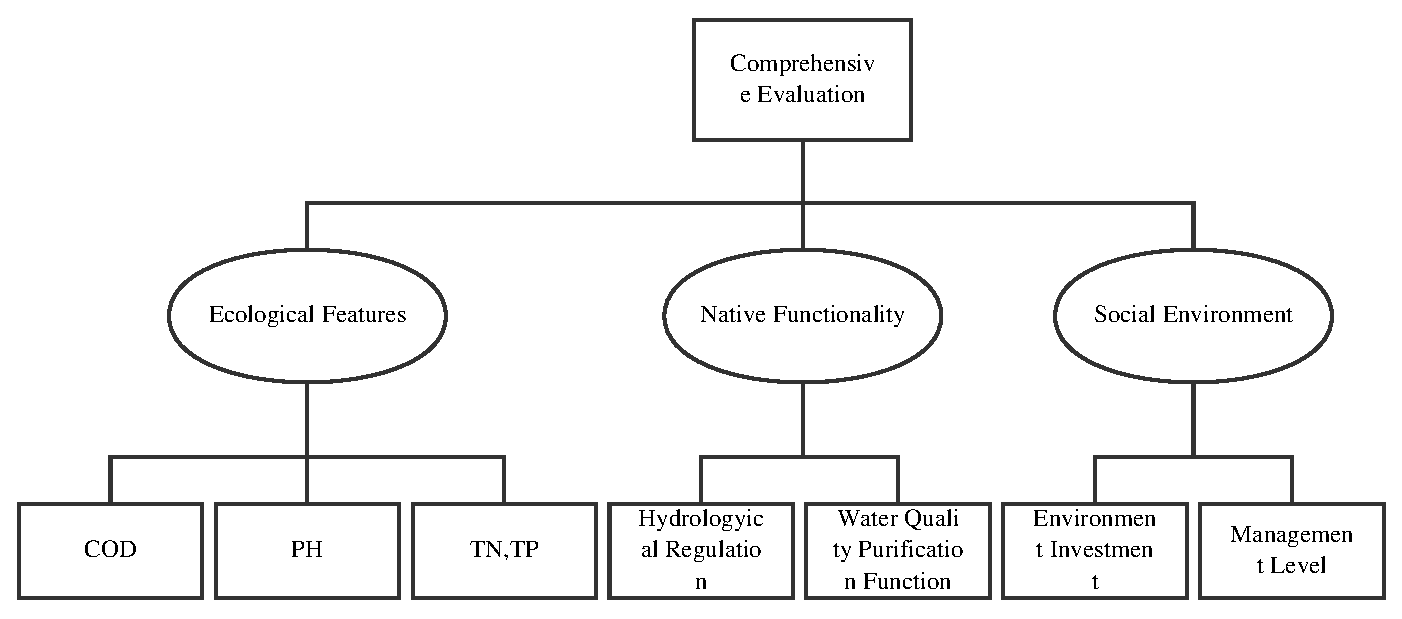
\includegraphics[width=\linewidth]{figure/AHP}
        \caption{AHP}
        \label{fig:AHP}
    \end{figure}
    
    
    % 构造指标间的判断矩阵
    \item[Step2] Constructing judgment matrix among factors.
    % 通过当地专家采用1~9标度打分,对各层因素两两间量化判断,可以得到相应的判断矩阵.
    We use the pairwise-comparison method and 1–9 method of AHP to get the corresponding judging matrix.
    % 层次单排序一致性检验
    \item[Step3] Consistency check of single hierarchical arrangement 
    % 定义CI为一致性指标.
    We define CI as Consistency index
    

\begin{equation}CI=\!\!\frac{\lambda_{max}-n}{n-1}\end{equation}

\begin{equation}CR=\frac{CI}{RI}\end{equation}
    
    
    %一般用CR值判断.当CR<0.1时,认为成对比较的逆对称矩阵可以接受.其中RI取值见下表:
    Generally, CR value is used to judge. When CR < 0.1, inverse symmetric matrices can be excepted. RI values can be seen in the following table:
    

%取值表
\begin{table}[h] \renewcommand\arraystretch{1.5}
    \begin{center}
        \begin{footnotesize}
            \begin{tabular}{ccccccccccc}\toprule[1pt]
                \it  n & \bf 1    &\bf 2     & \bf 3  & \bf 4   &\bf 5 & \bf 6 & \bf 7 & \bf 8 & \bf 9&\bf 10   \bigstrut\\\hline
                \it RI & 0.00 &0.00 &0.58 &0.90&1.12&1.24&1.32&1.45&1.51&1.41\bigstrut\\\bottomrule[1pt]
            \end{tabular}
        \end{footnotesize}
        \caption{\footnotesize {The values of RI}}
    \end{center}
\end{table}
    
    % 层次总排序及组合一致性检验
    \item[Step4] Consistency check of total taxis of hierarchy.
    %设上一层A包含m个因素A1,A2,,,Am.A的层次总排序权值分别为a1,,,am.下一层B包含n个因素B1,,,Bn.这些因素对于Aj的层次单排序的权值分别为b1j,,,bnj.那么,此时B层的总排序权值如下表所示:
    Level $A$ has m indexes like $A_1,A_2 \cdots A_m$, and the weights of A total taxis of hierarchy are $a_1, \cdots, a_m$. Level $B$ includes $n$ indexes like $B_1 \cdots B_n$.
    Eventually, we could get the weight of $B$'s total taxis of hierarchy which can be seen in the below according to the $A$ level single hierarchical arrangement.
    
    总排序表
    
    % 层次总排序一致性检验为:
    We get consistency check of total taxis of hierarchy
    
    \begin{equation}
    CR=\displaystyle\frac{\sum\limits_{j=1}^{m}a_jCI_j}{\sum\limits_{j=1}^{m}a_jRI_j}
    \end{equation}
    
    % 当CR<0.1时,认为层次总排序的结果具有满意的一致性.
    % 最终得到的评价模型为:
    When $CR < 0.1$, the results of total taxis of hierarchy satisfy the criteria.\\
    At last ,we can get:
    
    公式11
    
\end{itemize}\par

%4.1.2模型求解和结果分析
\subsubsection{Results and Analysis}
% AHP的排序结果如下表所示:
Finally, we can obtain the final rankings of the schools using the AHP model.

前几名的排序表

% 结果分析:
The analysis of conclusion:
% 我们得到的CR值为XX,可以认为排序结果具有满意的一致性.
The value of CR is, we draw a conclusion the result of ranking satisfies the criterion for consistency.Analyzing the weight vector of criteria level, the highest weight is for XXX指标.The weight of X指标 is the lowest.

%4.2 
\subsection{The calculation of the Return On Investment(ROI)}
%4.1.1 ROI定义
\subsubsection{The definition of ROI}
%在金融中,投资回报率指的是投资某个项目后所获得的收益的多少.而我们这道题目中,反映的是学生完成大学学业与否以及毕业后的情况.我们查阅相关文献资料了解在教育方面对ROI的理解.我们结合我们手中拥有的数据.我们给出ROI的定义如下: 
In financial terms, return on investment refers to the proportion of total profits obtained after investing one project. However, we define RIO as followed:

\begin{equation}
ROI = \frac{I - M}{M}
\end{equation}

\begin{equation}
I = n  \cdot [k \cdot Salary + (1-k) \cdot m]
\end{equation}

\begin{equation}
n = s \cdot g \cdot [P \cdot L_1 + (1-p) \cdot L_2]
\end{equation}

%其中,I表示毕业学生收入总和;n表示毕业学生人数;k表示6年后收入达到阈值的人数比例;m为毕业学生收入中位数;s表示招生人数;L_1表示兼职留校率,L_2表示非兼职留校率;p表示兼职率;g表示学校毕业率.
Where $I$, is the total revenue of graduated students; 
where $n$, is the total number of graduated students; 
where $k$, is the proportion of graduated students whose revenues reach threshold six years later; 
where $m$, is the median incomes of graduated students; 
where $s$ ,is the enrollments; 
where $L_1$ ,refers to part-time student retention rate; 
where $L_2$, refers to retention rate of students without jobs; 
$P$ refers to the proportions of part-time students; 
$g$ refers to graduation rate.

%4.2.2 ROI计算与验证
\subsubsection{The calculation of ROI and the validation of rankings}
%我们根据我们所建立的ROI计算公式,计算了若干学校的ROI指标,部分结果如下图:
We calculate ROI of all schools based on the formula of ROI, partial results are shown below:

学校与对应的ROI值表

从表中可以看出:
%层次分析法对主观因素依赖性较强.我们结合计算得到的各个学校的ROI值.综合考虑最终后,得到最终的投资候选名单为:
AHP is a subjective method. It largely depends on artificial scoring, so we calculate the ROI of every school to get the last rankings under the comprehensive consideration. The result is shown as followed:

投资候选名单,包含评价顺序一列,ROI值排序一列




%4.3持续时间模型
%\subsection{Duration-time Model}
%
%4.3.1模型的建立
%对于持续时间,我们通过计算不同年份的ROI随时间变化来确定.我们以The Ohio State University at Columbus学校为例,说明模型建立过程.
%Step1.收集学校信息
%我们从the U.S. National Center on Education Statistics收集了The Ohio State University at Columbus2007年到2010年的数据.
%Step2.计算ROI值
%通过整理、提取收集的数据,我们计算出07年至2010年各个年份对应的ROI值.
%Step3.曲线拟合分析
%我们将数据进行曲线拟合,图像如下:
%曲线拟合图
%通过图像我们可以了解到,学校的ROI值起伏变化.但是学校ROI的整体变化趋势是呈现递增的.所以我们对该学校投资时间越长越好.
%同样的道理,我们可以得到其他学校的投资持续时间.持续时间分布图如下:
%持续时间分布图

%4.4投资组合优化模型
\subsection{Optimal Model on Investment Combination}

%4.4.1金融领域的投资组合问题
\subsubsection{Investment Combination problem in the financial sector}
%投资,是指一定的经济主体将现期一定的收入转化为资产或资本以获得不确定的回报.其中广义的投资是指将资金投入风险领域以期获得较高回报的行为.狭义的投资是指投资者向新兴的、快速发展的或者高科技(有巨大的竞争潜力)企业投入股权资本,直接参与企业创业的行为.
Investment refers that economic agents transform certain income into assets or working capital to get the uncertain return. Moreover, generalized investment is an act of pumping the capital into risky area to get the high return, and narrowed investment is an act of participating in business venture.\par
%投资组合问题是金融学领域一个重要的课题.它主要研究如何在不确定的情况下对金融资产进行合理配置与选择,从而实现收益率最大化与风险最小化之间的均衡.1952年,经济学家Harry M.Markowitz在《The Journal of Finance》杂志上发表了"Portfolio Selection".Markowitz指出,理性的投资者总是寻求在给定期望收益水平的条件下,使风险最小的投资组合X.在该理论中,Markowitz用随机变量表示股票的价格,以它的均值来衡量收益.用随机变量的方差衡量风险,放映出收益的不稳定性.求给定风险下的最小风险或给定风险下的最大收益的投资组合问题,归结为一个线性约束下的二次规划问题.
Portfolio problem is an important topic in the field of finance. Its major research object is how to allocate the financial assets reasonably under the uncertainty to keep the balance between maximized yields and minimizing risks. Economist Harry M.Markowitz has pointed out that rational investor always seek the expectation for profit to minimize the risks of investment portfolio. He used the random variable as the price of stock , its mean to measure profit and the variance of a random variable to measure risks. Eventually, investment combinations problem under the minimal risks or given risks of maximum benefit can be boiled down the quadratic programming problem with linear constraints.\par
%设有n种风险资产.它们的收益率为随机变量R,协方差矩阵为V.其中ri表示第i种资产的随机收益率.投资组合为X=(...),xi表示投资者对第i种资产的投资比例.Markowitz的投资组合模型为:
We assume n kinds of risk assets. Their yields are random variable R and covariance matrices are v. $X=(x_1,x_2,\cdots,x_i)$ represents investment portfolio, so we can get 
$min \frac{1}{2}x^Tvx$	

\begin{equation}
s.t
\begin{cases}
E(\widetilde r^Tx)=E(R_p)\\
e^Tx=1
\end{cases}
\end{equation}

Where $r_i$, is the random rate of return ;
where $x_i$, is the proportion of i th asset for investors

%投资组合公式
%投资组合优化问题实际上是一个约束多目标优化问题.随着智能优化算法的提出及发展,智能优化算法被广泛应用于求解各类实际的工程问题,这也包括投资组合优化问题 .
Investment portfolio optimal problem is actually a constrained multiobjective programming.with the proposal of intelligent optimization algorithms, and they are widely applied into practical project, including portfolio optimization problem.Chen and Kou reported that400 publications are relevant to intelligent optimization algorithms applied in finance term, which are used to solve portfolio optimization problems$^{[\ref{3}]}$.


中指出,大约有 400 多种刊物的内容是关于智能优化算法在金融及经济学中的应用问题的,并且其中大多数是关于投资组合优化问题的.早期智能优化算法主要用于求解单目标无约束投资组合优化问题.Dueck 和 Winker

基于智能优化算法提出一个求解投资组合优化问题的局部搜索算法.Arnone 等

学者首先使用遗传算法求解投资组合优化问题$^{[\ref{4}]}$$^{[\ref{5}]}$.
\par

%4.4.2简化模型的建立
\subsubsection{The building of The Simplified Model}
%我们从简单情况入手,逐步靠近实际情况.我们假设投资的学校都投资五年.我们设xi表示投资的学校,其中xi满足:
We'll start with the simple situation,approaching actual conditions step by step. A bold assumption is proposed that the time of school we will invest is five years. Where $x_i$, is the school invested and satisfy:

\begin{equation}
x_i=
\begin{cases}
0,no investment\\
1,investment
\end{cases}
\end{equation}

Xi满足的式子
%wi表示投资给学校Xi的资金数目比例.我们类比MV模型,建立模型如下:
$w=i$ represents the proportion of the amount of money given to school $x_i$.we can get equations by imitating $MV$ model:

\begin{equation}
\begin{cases}
max\sum r_i\\
min\sum q_i\\
\sum\limits_{i=1}^{n}x_i\cdot w_i=1\\
q_i\cdot w_i\textless e
\end{cases}
\end{equation}

公式

%4.4.3动态多期投资组合模型建立
\subsubsection{Building Dynamic Multi - period Portfolio Model}
%我们考虑具体实际情况.设t表示投资期,t取值为1到5.Ait表示在第t个投资期给学习Xi投资的资金数.Z表示第t个投资期内投资的总资金.M表示总的投资资金.则建立模型如下:

复杂情况公式

We take actual situation into consideration, and then we can get 

\begin{equation}
\begin{cases}
max\sum r_{it}\\
min\sum q_{it}\\
\sum\limits_{i=1}^{n}x_{it}\cdot a_{it}=Z+B_{t-1}(1+r)
\end{cases}
\end{equation}

Where $t$, is the duration of investment and belongs to$[1,5]$; 
$a_{it}$represents the amount of investment on school $x_i$ at the t th investment period; $z$ presents the total capital at the $t$ th investment period.


\subsubsection{4.4.3简化模型的求解及结果分析}
%微粒群算法,又称粒子群优化(particle swarm optimization, PSO)是一类基于群体智能的随机优化算法.是由J. Kennedy和R. C. Eberhart等于1995年开发的一种演化计算技术.现已广泛应用于函数优化、神经网络训练、模式分类、模糊系统控制以及其他遗传算法的应用领域
Particle Swarm Optimization is a random optimization algorithm based on swarm intelligence, which is evolutionary computation technology, developed by J. Kennedy and R. C. Eberhart in 1995. Now, it is widely used in function, optimization neural network training and fuzzy control system$^{[\ref{6}]}$.\par

In the D –dimension search space, a group consists of n particles and i th particle refers to D-dimensional vectors, $x_i=(x_{i1},x_{i2},\cdots,x_{iD})^T,i=1,2,\cdots,n$. Then we plug $x_i$ back into a objective function to get its adaptive value. By comparing the size of value ,we can measure the strength and weakness.\par

The flight speed of i th particle should also be n dimensional vectors:

\begin{equation}
v_i=(v_{i1},v_{i2},\cdots,v_{iD})^T,i=1,2,\cdots,n
\end{equation}

But the speed of each dimension is limited the area $[-v_{max},v_{max}]$,$v_{max}$ determines the accuracy between current position and the best position. If $v_{max}$ is high, the particle may miss the optimal solution, on the contrary, if $v_{max}$ is too small, the particle will not explore insufficiently so as to be trapped in local optima.
The best position i th particle searched to date is:

\begin{equation}
p_i=(p_{i1},p_{i2},\cdots,p_{iD})^T,i=1,2,\cdots,n
\end{equation}

At the $n$ th iteration, the optimal location the particle swarm searched is:

\begin{equation}
p_g=(p_{g1},p_{g2},\cdots,p_{gD})^T,g=1,2,\cdots,m
\end{equation}

Before finding two optimal values, the particle swarm updates speed and position in the following equations;

\begin{equation}
\begin{cases}
v_{id}^{k+1}=w \times v_{id}^k+c_1r_1(p_{id}-x_{id}^k)+c_2r_2(p_{gd}-x_{gd}^k)\\
x_{id}^{k+1}=x_{id}^k+v_{id}^{k+1}
\end{cases}
\end{equation}

$i=1,2,\cdots,n$;$d=1,2,\cdots,D$;where $c_1$ and $c_2$, are learning factor and nonnegative number, which belong to $[0,2]$;$r_1$and $r_2$ are random numbers between 0 and 1;k refers to iteration.\par
%在利用粒子群算法时,为了简化问题,增加对粒子扩散的约束,主观因素引入一个参数e.则粒子群算法变为:
When using particle swarm algorithm,in order to simplify the problem and increase the confinement on the particle, so we introduce a subjective factor $e$.


\begin{equation}
\begin{cases}
v_{id}^{k+1}=w\times v_{id}^k+c_1r_1(p_{kl}-x_{kl}^k)+c_2r_2(p_{gd}-x_{gl}^k)\\
x_{id}^{k+1}=x_{id}^k+v_{id}^{k+1}\\
x_{id}^{k}\leqslant e
\end{cases}
\end{equation}

%参数设定如下:w的取值范围[0.8,1.0].常数c1,c2取值范围为[0,2].权重变化速度的界限常数vmax取值范围为[0,1]. e作为约束条件分别设置为(5,10,15,20,25,30,35,40,45,50),本实验结束条件为最大迭代次数600次.
Parameters are set as follows:
The range of w is 0.8 to1.0;The constant range is 0 to 2.where $v_max$, is the limit of speed and range from 0 to 1.
$e$ as condition of constraint is set $(5,10,15,20,25,30,35,40,45,50)$respectively. 
The number of iterations just only reach 600 times.


\begin{figure}[h]
    \centering
    \includegraphics[width=\linewidth]{"figure/relevant-variable-with-ROI"}
    \caption{Only "PCTPELL" is a relevant variable with ROI}
\end{figure}

%为了调整ROI定义对优秀大学的倾向性,我们对剩下四个可能有关系的变量与ROI做了相关性分析,结果除了"PCTPELL"有 0.46 的相关系数外,其他变量与ROI几乎不相关 
To adjust the definition of ROI to the tendency of good university,we do the correlation analysis with four variables affecting ROI.From the picture ,we can find that only "PCTPELL" have 0.46 correlation coefficient  and the others have nothing to do with ROI.so, we do not adjust the formula of ROI.\par

结果分析(待定)

%5.灵敏性分析
\section{Sensitivity Analysis}
%5.1 ROI定义式的灵敏性分析
\subsection{The sensitivity analysis of the definition of ROI}
%在实际情况中,很多因素我们是有很大不确定性的.我们计算ROI对毕业生的工资(题目所给数据中的一项指标)的灵敏性程度.我们记ROI为r,则得到:

公式

In the actual situation,many factors exist considerable uncertainty. We can get the degree of sensitivity between graduated students' income and ROI by calculating and define ROI as r, then we get  

$$S(r,m)=\frac{dr}{dm}\cdot\frac{m}{r}=1.6$$

%由公式可以看出来,工资每增加10%, 学校的ROI提高16%.ROI定义式对工资具有较好的稳定度.因为我们所定义的ROI是毕业学生的社会贡献程度.而工资水平放映了他一定的贡献度.
From the equation, we can explicitly see that the ROI improves 16\% when the income increases 10\% in per, which reflect the good stability of income in terms of
ROI definition, because the ROI we define is the degree of contributions to society for students. Coincidently, wage can show contributions to some extent.
\par

\subsection{5.2简化模型的灵敏性分析}
%实际投资中,我们面临的投资学校数目将是巨大的.我们分析投资结果对可投资数目的灵敏性.通过增加数目,粒子群算法收敛性越来越差.这个情况说明的我们的模型稳定性很差.需要进一步分析约束条件的设定.
In the actual investment, we will have to solve more schools to invest. We analyze the sensitivity of the investment results about the numbers of schools. The convergence of PSO becomes worse and worse with the numbers increasing. This result indicates that the stability of our model is poor. We need future work to improve our model.\par

%6.模型评价
\section{Model analysis}
%优点
\subsection{Strength}
%我们对数据分析的较为透彻.我们仔细分析了数据类型及性质.理解了"null"值出现的原因,有效的解决了问题.
We have a clear understanding of data by analyzing data types and properties and know the reason why "NULL" appears, solving the problem effectively.
%我们将问题分解为几个子问题求解,将问题细化.我们一共建立了三个模型,分别用于求解投资学校、投资金额以及持续时间.模型之间相互联系,共同构成一个整体.
We further classify a problem into some small problems and build three models, which are used in identifying investment schools, investment amount and duration time. The models interconnect mutually and constitute a whole. 
%合理提出假设,并初步细化模型.我们通过提出合理的假设,简化问题的分析.然后逐步建立复杂模型,逼近真实情况.
Reasonable assumptions are proposed properly and the models are break down. We firstly simplify the analysis of the problem by coming up with reasonable assumption. Then we build the more complex model step-by-step to approach the real situation.

%缺点
\subsection{Weakness}
%定义的ROI考虑不全面.我们只考虑了与ROI最直接相关的因素.所以,对于ROI的定义不够准确,在一定程度上无法反映各个大学真是的回报率.
We consider the factors uncomprehensive when we define the ROI. We only take into account the directly factors. So the definition we propose is inaccurate. It is not able to reflect the real ROI of each university.
%数据处理主观判断影响较大.通过对题目给的数据以及收集的数据的整理,我们主观舍弃了一些没有价值的指标.使我们最后分析的结果有一定影响.
The subjective judgment influences the data processing a lot. Through sorting out the data the problem provides or we collect, we abandon some indexes subjectively. It may lead to some effect on the results.
%AHP评价结果受主观因素影响较大,不够准确.
The results getting from the AHP are easily influenced by the subjective judgment. 
%持续时间估算的不够准确.由于学校不同年份的数据较少,每个学校只有4到5年的数据.根据图像走势作出的判断不够准确.
The time duration is not inaccurate. Because the data of schools for each year are little. There only are four or five years data for each school. So the time duration we estimate is unreliable.
\subsection{Future work }
%完善对ROI的定义.进一步分析数据,找出所有与ROI相关的因素.建立更能够反映学校回报率的ROI定义.优化投资策略.
We need to complete the definition of ROI. We need analyze the data more deeply to find all the factors related ROI. Then we define the ROI again.
%结合模糊综合评价,降低AHP的主观性的影响.模糊综合评价更依赖于数据.整合两种评价方法,选取恰当的权值比例.能够有效地减少AHP的主观因素影响.这样可以进一步优化候选名单.
We could combine the Fuzzy Comprehensive Evaluation(FCE). FCE is an objective method, it depends on data. To comprehensively consider the effect of subjective and objective factors, we can improve the reliability of our results.
%完善动态的多期的投资组合模型.多期多目标动态投资组合模型,考虑情况更加接近实际情况.通过这个模型,可以在统一分析投资资金、投资学校和投资时间的情况下求解各值.
We need to complete the portfolio investment dynamic model. This model takes all the relation into consideration to increase the reliability of our results. 

%文献引用
\begin{thebibliography}{99}
    \bibitem{1} The Quest for Societal ROI in the Midst of the Perfect Storm:Can SCM Set the Standard for Twenty-First Century Business Education? Journal of Business Logistics, 2015, 36(1): 1–8\label{1}
    \bibitem{2} The Economist. 2014b. "Higher Education: Creative Destruction." The Economist (June 28). http://www.economist.com/news/leaders/21605906-cost-crisis-changing-labour-markets-and-newtechnology-will-turn-old-institution-its—The Economist (2014b)\label{2}
    \bibitem{3}  Chen S. H. , Kuo T. W. . Evolutionary computation in economics and finance: a bibliography.  Evolutionary  computation  in  economics  and  finance. Physica-Verlag, Heidelberg, New York, 2002. 419-455.\label{3}
    \bibitem{4} Dueck  G.  ,  Winker  P.  .  New  concepts  and  algorithms  for  portfolio  choice. Applied Stochastic Models and Data Analysis. 1992, 8(3), 159-178.\label{4}
    \bibitem{5} Arnone  S.  ,  Loraschi  A.  ,  Tettamanzi  A.  .  A  genetic  approach  to  portfolio selection.  Neural  Network  World:  International  Journal  on  Neural  and Mass-Parallel Computing and Information Systems. 1993, 3(6), 597-604.\label{5}
    \bibitem{6} 曾建潮,介婧,崔志华.微粒群算法[M].北京:科学出版社,2004:9- 13\label{6}
    
\end{thebibliography}

\newpage
% 信件
Dear Mr. Alpha Chiang:\\
We identified an optimal investment strategy which identifies schools, investment amount per school, return on that investment(ROI), and time duration during these days. Now, let me tell you our modeling approach and major results.\par
The first step was to analyze and process the data the problem provides. It appears a number of ''NULL'' results, which is defined as the lack of properties in some schools rather than missing data. We employed Principal Component Analysis (PCA) to reduce dimensions of big data and get some principal components. Then combining with ROI and funds utilization, we can formulate an evaluation model based on Analytical Hierarchy Process (AHP) to obtain the primary list of candidate schools.\par
Then we defined the ROI. We regard ROI as the degree of graduates’ contributions to the society. Combining with the data we capture, we define a formula for ROI. The data which is related to ROI have income, academic achievement and so on. We processed the data by different types we classified. We imitated the ROI in the financial sector to get our “ROI”. The result is showed as follows:

ROI定义式
符号说明

We calculated the ROI of every school. We used the results to test the results we have gotten from AHP. The compared results were showed as follows:

两个方法部分结果对比

We build an investment portfolio optimization model to determine the investment schools and the investment amount per school with hybrid particle swarm algorithm(PSO). In order to analyze the problem explicitly, we build a basic model. We hypothesis that the time duration for investment of all schools is all five years. Then we formulate a multi-objective optimization model for the aim of getting the maximum return. Through the method of PSO, We extend our model with taking the change of time duration into consideration. We divide the time duration into five parts. The time duration of each school decides on its ROI. The relationship among variables becomes more complicate. So we build a portfolio investment dynamic model. This model takes all the relation into consideration to increase the reliability of our results. \par
Eventually, we present the investment strategy is as follows:

结果表格


%附录
\begin{appendices}
    
    \section{Ranking Table}
    
    
    %\input{rank_table.tex}
    \begin{tabular}{lcc}\hline
        INSTNM	 &FINIANCE	&TIME\\\hline
        Ohio State University-Main Campus	&110	&3\\
        Texas A M University-College Station	&&110	3\\
        Pennsylvania State University-Main Campus	&110&	3\\
        The University of Texas at Austin	&110&	3\\
        University of Central Florida	&110	&3\\
        University of California-Los Angeles	&110	&3\\
        University of Florida	&110&	3\\
        Michigan State University	&110	&3\\
        University of California-Berkeley	&110&	3\\
        University of Illinois at Urbana-Champaign&	110&	3\\
        University of Michigan-Ann Arbor	&110	&3\\
        Rutgers University-New Brunswick	&110	&3\\
        University of Wisconsin-Madison&	110&	3\\
        University of California-Davis	&110	&3\\
        University of Washington-Seattle Campus&	110&	3\\
        Indiana University-Bloomington	&110	&3\\
        University of California-San Diego	&110	&3\\
        Florida State University	&110	&3\\
        Brigham Young University-Provo	&110	&3\\
        University of Maryland-College Park	&110	&3\\
        University of California-Irvine	&110	&3\\
        University of Georgia	&110	&3\\
        University of Minnesota-Twin Cities	&110&	3\\
        Purdue University-Main Campus&	110	&3\\
        New York University	&80	&2\\
        Virginia Polytechnic Institute and State University&	80&	2\\
        Arizona State University-Tempe	&80&	2\\
        University of Southern California	&80&	2\\
        California State University-Long Beach	&80&	2\\
        The University of Alabama	&80&	2\\
        Temple University	&80&	2\\
        San Diego State University	&80	&2\\
        Iowa State University	&80&	2\\
        University of California-Santa Barbara	&80&	2\\
        University of North Carolina at Chapel Hill&	80&	2\\
        University of Arizona	&80	&2\\
        University of Missouri-Columbia	&80	&2\\
        California State University-Fullerton	&80	&2\\
        University of Colorado Boulder	&80	&2\\
        Florida International University	&80&	2\\
        North Carolina State University at Raleigh	&80	&2\\
        University of South Florida-Main Campus&	80&	2\\
        University of South Carolina-Columbia	&80	&2\\\hline
    \end{tabular}
    
    \newpage
    \begin{tabular}{lcc}\hline
        Texas Tech University	&38	&1\\
        Clemson University	&38&	1\\
        University of Pittsburgh-Pittsburgh Campus	&38	&1\\
        University of Iowa	&38	&1\\
        Texas State University	&38&	1\\
        George Mason University	&38&	1\\
        University at Buffalo	&38	&1\\
        Colorado State University-Fort Collins	&38	&1\\
        California State University-Northridge	&38	&1\\
        Auburn University	&38&1\\
        University of California-Riverside	&38&	1\\
        University of Utah	&38&	1\\
        University of Houston	&38	&1\\
        Washington State University	&38&	1\\
        University of Oregon	&38	&1\\
        The University of Tennessee-Knoxville	&38&	1\\
        Miami University-Oxford	&38	&1\\
        Syracuse University	&38	&1\\
        Georgia Institute of Technology-Main Campus	&38&	1\\
        Oregon State University	&38&	1\\
        University of California-Santa Cruz	&38&	1\\
        University of North Texas	&38	&1\\
        San Jose State University	&38	&1\\
        Grand Valley State University	&38&	1\\
        University of Oklahoma-Norman Campus	&38	&1\\
        Towson University	&38	&1\\
        University of Cincinnati-Main Campus&	38	&1\\
        Liberty University	&38&	1\\
        California State Polytechnic University-Pomona	&38&	1\\
        Northeastern University&	38	&1\\
        University of Virginia-Main Campus	&80	&2\\
        University of Connecticut	&80	&2\\
        University of Massachusetts-Amherst	&80&	2\\
        Cornell University	&80	&2\\
        James Madison University	&80&	2\\
        Louisiana State University and Agricultural Mechanical College&	80	&2\\
        Boston University	&80	&2\\
        University of Delaware	&38	&1\\
        California Polytechnic State University-San Luis Obispo	&38	&1\\
        SUNY at Binghamton	&38&	1\\
        Ohio University-Main Campus&	38	&1\\
        Virginia Commonwealth University	&38	&1\\
        University of Nebraska-Lincoln	&38	&1\\
        Miami Dade College	&38	&1\\
        Illinois State University	&38	&1\\
        University of Kentucky	&38	&1\\\hline
    \end{tabular}
    
    \newpage
    \begin{tabular}{lcc}\hline
        University of Pennsylvania&	38	&1\\
        University of Arkansas	&38	&1\\
        Stony Brook University&	38	&1\\
        West Virginia University	&38&	1\\
        
        Drexel University	&38&	1\\
        Georgia State University	&38&	1\\
        University of Kansas&	38	&1\\
        DePaul University	&38&	1\\
        San Francisco State University&	38&	1\\
        Oklahoma State University-Main Campus	&38&	1\\
        
        California State University-Sacramento	&38	&1\\
        Kansas State University	&38&	1\\
        Baylor University	&38&	1\\\hline
        East Carolina University	&38	&1\\
        Appalachian State University	&38	&1\\
        University of Miami	&38	&1\\
        University of North Carolina at Charlotte	&38	&1\\
        Central Michigan University	&38	&1\\
        De Anza College	&38	&1\\
        Montclair State University	&38&	1\\
        University of New Hampshire-Main Campus&	38	&1\\
        Boston College	&38&	1\\
        Northwestern University	&38&	1\\
        California State University-Fresno&	38&	1\\
        Kent State University at Kent	&38	&1\\
        Columbia University in the City of New York	&38&	1\\
        CUNY Bernard M Baruch College	&38&	1\\
        University of Notre Dame	&38	&1\\
        University of Illinois at Chicago	&38	&1\\
        Western Washington University	&38&	1\\
        Valencia College	&38	&1\\
        West Chester University of Pennsylvania	&38	&1\\
        University of Mississippi	&38	&1\\
        George Washington University	&38	&1\\
        California State University-Chico	&38&	1\\
        Western Michigan University&	38	&1\\
        Florida Atlantic University	&38&	1\\
        Rochester Institute of Technology	&38	&1\\
        Brigham Young University-Idaho&	38	&1\\
        Mississippi State University	&38	&1\\
        Old Dominion University	&38	&1\\
        Harvard University	&38	&1\\
        CUNY Queens College	&38	&1\\
        University of New Mexico-Main Campus	&38	&1\\
        Northern Arizona University&	38	&1\\
        SUNY at Albany	&38&	1\\
        Stanford University	&38	&1\\
        The University of Texas at Dallas	&38	&1\\
        Ball State University	&38	&1\\
        Emory University	&38&	1\\
        University of North Carolina Wilmington	&38	&1\\
        Northern Virginia Community College&	38	&1\\
        Georgia Southern University	&38	&1\\
        The University of Texas at Arlington	&38	&1\\
        University of Rhode Island	&38	&1\\
        Kennesaw State University	&38	&1\\\hline
        
    \end{tabular}
    
    
    \newpage
    \begin{tabular}{lcc}\hline
        Georgetown University	&38&	1\\
        Western Governors University	&38&	1\\
        University of Vermont	&38&	1\\
        Washington University in St Louis	&38	&1\\
        CUNY Hunter College&	38&	1\\
        Vanderbilt University	&38	&1\\
        Utah State University	&38&	1\\
        Orange Coast College	&38&	1\\
        Fordham University	&38	&1\\
        Pasadena City College	&38	&1\\
        University of Nevada-Las Vegas	&38	&1\\
        Rowan University	&38&	1\\
        Duke University&	38	&1\\
        Mt San Antonio College	&38	&1\\
        University of Nevada-Reno	&38&	1\\
        University of Maryland-Baltimore County	&38&	1\\
        Broward College	&38	&1\\
        University of Hawaii at Manoa	&38	&1\\
        Brown University	&38	&1\\
        California State University-San Bernardino	&38	&1\\
        University of Wisconsin-Milwaukee	&38	&1\\
        Princeton University	&38	&1\\
        Villanova University	&38	&1\\
        Missouri State University-Springfield	&38&	1\\
        Texas Christian University	&38	&1\\
        California State University-Los Angeles&	38	&1\\
        Middle Tennessee State University	&38	&1\\
        Sam Houston State University	&38	&1\\
        Marquette University	&38	&1\\
        Indiana University-Purdue University-Indianapolis	&38&	1\\
        University of Chicago	&38	&1\\
        Loyola University Chicago	&38	&1\\
        College of William and Mary	&38	&1\\
        Southern New Hampshire University	&38	&1\\
        St John's University-New York	&38	&1\\
        Northern Illinois University	&38&	1\\
        East Los Angeles College	&38	&1\\
        Yale University	&38	&1\\
        University of Louisville	&38	&1\\
        Johns Hopkins University	&38	&1\\
        CUNY Brooklyn College	&38	&1\\
        College of Charleston	&38	&1\\
        
        
        \hline
    \end{tabular}
    
    \begin{tabular}{lcc}\hline
        University of Dayton	&38	&1\\
        Bowling Green State University-Main Campus	&38	&1\\
        University of Wisconsin-Eau Claire	&38	&1\\
        Portland State University	&38&	1\\
        Indiana Wesleyan University	&38	&1\\
        The College of New Jersey	&38&	1\\
        Santa Monica College	&38	&1\\
        Tulane University of Louisiana	&38&	1\\
        University of North Florida	&38&	1\\
        University of Wisconsin-La Crosse 	&38	&1\\
        University of Rochester	&38&	1\\
        University of North Carolina at Greensboro	&38&	1\\
        University of Northern Iowa	&38&	1\\\hline
        
    \end{tabular}
    
    
    \section{Second appendix}
    
    some more text \textcolor[rgb]{0.98,0.00,0.00}{\textbf{Input C++ source:}}
%    \lstinputlisting[language=C++]{./code/mcmthesis-sudoku.cpp}
    
\end{appendices}

\end{document}